% !TEX root = ../Hamiltonian_of_mean_force.tex
\section{Physical regimes of the mean-force state}
\label{sec:physical_regimes}
Even in this simple case, the physics encoded in the mean force state by its dependence on temperature and bath coupling is startlingly rich. To expose this, we first commit to a specific bath spectral density for numerics.  We choose
the Ohmic spectral density
\begin{equation}
  J(\omega) = \alpha\,\omega\,e^{-\omega/\omega_c},
  \qquad \omega\in[0,2\omega_q],
  \label{eq:J_ohmic}
\end{equation}
with $\alpha=1$ and $\omega_c = 5\omega_q$. Unless otherwise stated, we further specialise to $\theta=\pi/4$
throughout.  We emphasise here that the choice of spectral shape is not fundamental,
as it only controls the way in which $\chi$ runs
with temperature. 

This apparently innocuous expression encodes the entire non-perturbative recombination of bare Hamiltonian and influence, and functions as an \emph{order} parameter for the crossover between weak and strong coupling regimes. The reduced equilibrium state transitions between these regimes as $\chi$ passes through unity,
\begin{equation}
    \chi(\beta,g,\theta)\sim 1
    \qquad \Longleftrightarrow \qquad
    g^2 \sim \chi_0(\beta,\theta)^{-1}.
    \label{eq:chi_crossover_condition_v5}
\end{equation}



This crossover condition $\chi(\beta,g,\theta)=1$ therefore
defines a coupling-dependent temperature scale
\begin{equation}
  g_\star(\beta) = \chi_0(\beta,\theta)^{-1/2},
  \label{eq:gstar_def_v6}
\end{equation}
and an equivalent crossover temperature $\beta_\star(g)$. Notably, these dual crossover values are an exact property of the solution.

The function $\gamma(\chi)$ is elementary but worth dwelling on. It is monotone decreasing
from $\gamma(0)=1$ to $\gamma(\infty)=0$ with its inflection near $\chi\approx
1.2$, and admits clean asymptotic forms:
\begin{align}
  \chi \ll 1:\quad &\gamma \simeq 1 - \tfrac{\chi^2}{3}
    \quad\text{(weak coupling)},  \label{eq:gamma_weak}\\
  \chi \gg 1:\quad &\gamma \simeq \chi^{-1} = (g^2\chi_0)^{-1}
    \quad\text{(ultrastrong)}.   \label{eq:gamma_strong}
\end{align}
In the weak-coupling regime the state tracks the bare Gibbs thermal state with
$O(g^2)$ corrections, as expected. Notably, as shown in Fig.~\ref{fig:chi_theory}, the crossover between regimes depends on \emph{both} temperature and coupling strength. This means that two distinct regimes emerge in the limit of scaling $g$ and $\beta$, wholly dependent on which side of the crossover is taken. 

Notably, these critical temperatures and couplings have an \emph{involutive} relationship, in the sense that
\begin{equation}
    \beta_\star(g_\star(\beta)) = \beta, \quad g_\star(\beta_\star(g)) = g.
    \label{eq:involutive_relationship}
\end{equation}
This relationship between temperature and coupling means the crossover can be interpreted as the \emph{self-dual} line in the $(\beta, g)$ plane, as explored in Fig.~\ref{fig:involutive_map}. This line represents a coupling-dependent temperature scale $\beta_\star(g)$ (or equivalently $g_\star(\beta)$), where different parameter scaling relationships apply.

\begin{figure}[t]
  \centering
  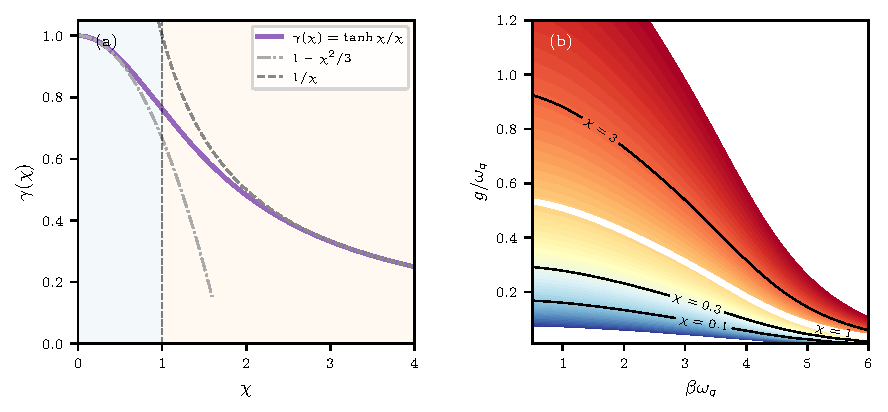
\includegraphics[width=0.48\textwidth]{../figures/hmf_fig1_chi_theory_ab.pdf}
  \caption{Universal crossover for the qubit mean-force state.
    \textbf{(a)} Crossover function $\gamma(\chi)=\tanh\chi/\chi$ interpolating
    between the weak-coupling approximant $1-\chi^2/3$ and the ultrastrong form
    $1/\chi$.  Shaded regions mark the weak (blue) and strong (orange) regimes
    separated by $\chi=1$.
    \textbf{(b)} Dimensionless coupling $\chi(\beta,g) = g^2\chi_0(\beta)$ as a
    contour map.  Vertical trajectories (fixed $g$) will crossover at its corresponding
    $\beta_\star(g)$.}
  \label{fig:chi_theory}
\end{figure}

\begin{figure}[t]
    \centering
    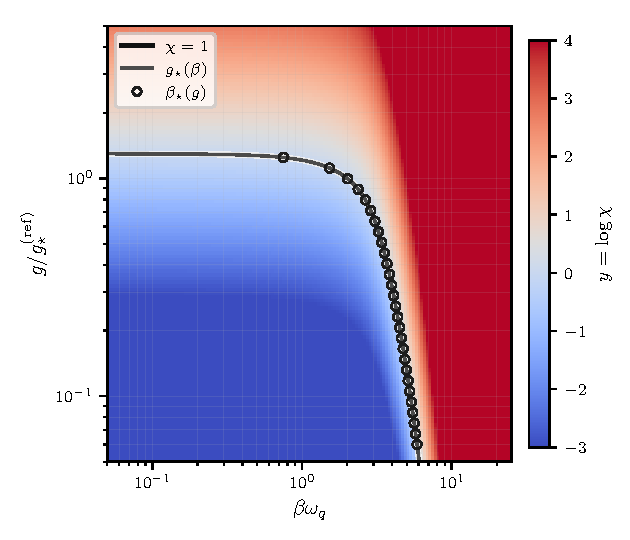
\includegraphics[width=0.48\textwidth]{../figures/hmf_crossover_involutive_v1.pdf}
    \caption{Involutive crossover geometry generated by $\chi(\beta,g) = g^2\chi_0(\beta)$. 
    The heatmap shows $y = \log\chi$ in the $(\beta, g)$ plane. The solid black line marks the crossover locus $\chi=1$, which can be constructed either as a coupling-dependent temperature $\beta_\star(g)$ (circles) or a 
    temperature-dependent coupling $g_\star(\beta)$ (solid grey line). This involutive relationship defines a partition between the weak-coupling (blue) and strong-coupling (red) scaling regimes.}
    \label{fig:involutive_map}
\end{figure}

\subsection{State purity}
\label{subsec:purity}
The purity of the reduced qubit state is
\(\mathcal{P}_Q = \tfrac{1}{2}(1+r_Q^2)\), with \(r_Q^2=|\mathbf r_Q|^2\).
From this we can immediately establish a universal result in the direct representative:

\begin{quote}
\textbf{Direct-representative bath purification.}\; \textit{For any positive spectral density
$J(\omega)\geq 0$ and any $\beta>0$: (i) $r_Q^2(g,\beta)$ is strictly increasing
in $g$ for $g\geq 0$, and (ii) for all $g>0$,}
\begin{equation}
    r_Q^2(g,\beta) \;>\; r_0^2(\beta) \;\equiv\; \tanh^2\!\left(\frac{\beta\omega_q}{2}\right),
    \label{eq:purity_bound}
\end{equation}
\textit{with equality only at $g=0$.}
\end{quote}

\paragraph{Proof sketch.}
Part~(i) follows immediately from
\(r_Q=\tanh\chi=\tanh(g^2\chi_0(\beta))\): since \(\tanh\) is strictly increasing and
\(g^2\chi_0\) is strictly increasing in \(g\), so is \(r_Q\).

Part~(ii) (excess over bare) uses the non-negativity of the resonant (longitudinal) dressing $\Sigma_z$. From the explicit integral form of the response kernels (cf.\ App.~\ref{app:qubit_ladder_derivation}), one has
\begin{equation}
    \Sigma_z = \frac{1}{\pi}\int_0^\beta u(\beta-u)\,K(u)\,\frac{\sinh(\omega_q u)}{u}\,du.
\end{equation}
Since $K(u)\geq 0$ for a physical spectral density, and the remaining factors are non-negative on the integration domain, we have $\Sigma_z > 0$ for all $\beta>0$. 

Substituting the exact components \(m_z=\tanh\Theta\) and \(m_\perp\) from
Eq.~\eqref{eq:bloch_locking_linear}, the purity excess
\(\Delta r_Q^2=r_Q^2-\tanh^2(\beta\omega_q/2)\) is strictly positive whenever
\(\gamma s^2\Sigma_z>0\). Physically, the longitudinal bath channel reinforces
polarisation and raises purity above the bare value. \(\square\)

In the limit $\beta\to 0$ (infinite temperature), the bare state is maximally mixed, yet the
mean-force state has
\begin{equation}
    r_Q\big|_{\beta\omega_q\to 0} = \tanh\chi > 0,
    \label{eq:purity_highT}
\end{equation}
This result is independent of the bandwidth or spectral shape of $J(\omega)$:
widening the bath increases $\chi_0(\beta)$ (driving the crossover to weaker
$g$) but cannot reverse the purity inequality.  Purity inversion would require
reversing the sign of the longitudinal response ($\Sigma_z < 0$), which is impossible for
any physical (positive) spectral density. 

Figure~\ref{fig:purity_figure} confirms this numerically. Panel (a) shows
\(r_Q(g/g_\star)\) for four temperatures. Every trajectory lies strictly above
its own \(r_0\) reference line for all \(g>0\), confirming Eq.~\eqref{eq:purity_bound}.
Panel (b) shows \(\Delta r_Q^2=r_Q^2-\tanh^2(\beta\omega_q/2)\) over the full \((g,\beta)\) plane.
Enhancement peaks at large \(g\)
and high temperature (upper-right corner), and falls to near zero at low
temperature (left edge) where the bare state is already nearly pure.  The black dashed contour $\chi=1$ marks the crossover at which purification
accelerates steeply.

This statement needs one caveat. It applies to the \emph{direct}
representative \((\beta,g)\). Under the strong--weak representative involution
\(g^\vee=g_\star^2/g\), one has \(\chi^\vee=1/\chi\), so
\begin{equation}
    r_Q^\vee(\beta,g)=\tanh(\chi^\vee)=\tanh(1/\chi).
    \label{eq:purity_dual_representative}
\end{equation}
Hence a highly pure direct strong-branch point maps to a weak-branch dual point
with reduced \(r_Q^\vee\). This is representative duality, not a contradiction
of Eq.~\eqref{eq:purity_bound} at fixed physical parameters.

\begin{figure}[t]
    \centering
    
\includegraphics[width=\columnwidth]{../figures/hmf_purity_figure.pdf}
    \caption{Purity of the qubit mean-force state.
    \textbf{(a)} Reduced-state Bloch radius \(r_Q\) versus scaled coupling \(g/g_\star(\beta)\)
    for four temperatures.  Dotted horizontals show the bare thermal purity
    \(r_0 = \tanh(\beta\omega_q/2)\); coupling always increases purity
    (Eq.~\eqref{eq:purity_bound}), most visibly at high temperature where the
    bare state is near-maximally-mixed.  Shaded regions mark the weak (blue) and
    strong (orange) coupling regimes.
    \textbf{(b)} Purity excess \(\Delta r_Q^2 = r_Q^2 - \tanh^2(\beta\omega_q/2)\) in the
    $(g,\beta)$ plane.  The black dashed contour marks the crossover locus
    $\chi=1$: purification is strongest at large $g$ and high temperature and
    saturates as \(r_Q\to 1\) deep in the strong-coupling regime.}
    \label{fig:purity_figure}
\end{figure}

\begin{figure}[t]
    \centering
    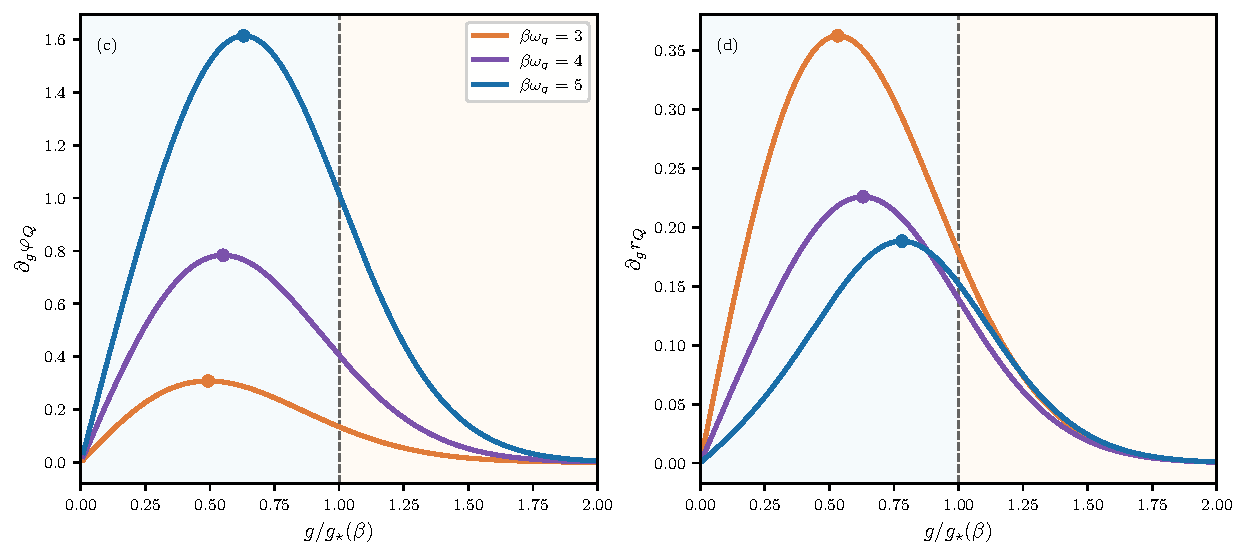
\includegraphics[width=0.48\textwidth]{../figures/hmf_fig1_chi_theory_cd_v3.pdf}
    \caption{Coherence and purity susceptibilities.
    \textbf{(c)} Reduced-state tilt susceptibility \(\partial_g\varphi_Q\) versus scaled
    coupling $g/g_\star(\beta)$ for three temperatures.  Rescaling collapses the
    peak positions to a universal value $g/g_\star \approx 0.65$, marked by filled
    circles.
    \textbf{(d)} Purity gradient \(\partial_g r_Q\); the rescaled peak occurs at
    $g/g_\star \approx 0.92$.}
    \label{fig:chi_susceptibility}
\end{figure}

\subsection{Quantum enhancement of heat engines}
An important feature of the crossover regime is that it demarcates where the
state is maximally sensitive to bath coupling. This is seen by considering
\(\partial_g\varphi_Q\) and \(\partial_g r_Q\), which quantify how rapidly the
Bloch vector tilts and purifies per unit change in \(g\). As
Fig.~\ref{fig:chi_susceptibility} shows, both peak near the
crossover $\chi =1$. $\partial_g\varphi_Q$ maximises at $g \approx 0.65\,g_\star$
(at $\chi_{\rm peak,\varphi}\approx 0.42$) and $\partial_g r_Q$ maximises at $g
\approx 0.92\,g_\star$ ($\chi_{\rm peak,r}\approx 0.85$).  The locations are
approximately pinned at universal values of $\chi$ independent of temperature, as demonstrated by the alignment of peaks when plotted as a function of the rescaled coupling $g/g_\star(\beta)$. The crossover region $\chi\sim 1$ is therefore where bath coupling yields the
greatest rate of return: both the onset of coherence (tilt of the Bloch vector
away from the bare thermal axis) and the onset of purification are most rapid
here, before both effects saturate as $\chi\to\infty$.  This suggests the
crossover regime is the most operationally leveragable for state engineering. 

We can immediately demonstrate this phenomenon with a toy model of a heat engine. In particular, we consider an Otto-stroke cycle, with unitary strokes. This can extract at most the system
\emph{ergotropy} per stroke with respect to the stroke Hamiltonian. The ergotropy of a state $\rho$ with respect to $H_Q$ is

\begin{equation}
  W_{\rm erg}(\rho,H_Q)
  = \Tr(\rho H_Q) - \min_{U}\Tr(U\rho U^\dagger H_Q),
  \label{eq:ergotropy_def}
\end{equation}

where the minimisation is over all unitaries \(U\). For any qubit the
minimiser is a \emph{passive rearrangement}. The Bloch vector is simply rotated
antiparallel to the ground direction $-\hat{\mathbf{n}}_s$ of $H_Q$ at
fixed spectrum. The passive state has Bloch vector
\(\vec{m}^{\,\rm pas}=-r_Q\hat{\mathbf n}_s\) and energy
\(-\omega_q r_Q/2\).

To expose the coherence contribution explicitly, define the incoherent
reference \(\delta[\rho]\equiv\operatorname{diag}(\rho)\) in the \(H_Q\)
eigenbasis. The coherence-enabled contribution is
\begin{equation}
\begin{split}
  \delta W_{\rm coh} &:= W_{\rm erg}(\rho,H_Q)-W_{\rm erg}(\delta[\rho],H_Q) \\
  &= \frac{\omega_q}{2}\!\left(\sqrt{m_z^2+m_\perp^2}+m_z\right), \qquad m_z\le 0,
\end{split}
\label{eq:delta_W_coh}
\end{equation}

Both equalities in Eq.~\eqref{eq:delta_W_coh} warrant justification.
The physics decomposes cleanly into two independent structural facts. First, \emph{the dephased state is always passive}. Energy dephasing leaves a diagonal state $\delta[\rho]$ with populations
$p_\pm = (1\pm m_z)/2$.  For $\delta[\rho]$ to be passive one needs the
larger eigenvalue on the lower-energy level, i.e.\ $p_- \geq p_+$, which
reduces to $m_z \leq 0$.  This is guaranteed by the bath: $\Sigma_z > 0$
for any positive spectral density (established in Sec.~\ref{subsec:purity}),
which forces $m_z < 0$ at all finite $g$ and $\beta$.  An incoherent cycle
running on $\delta[\rho]$ therefore extracts zero work,
$W_{\rm erg}(\delta[\rho],H_Q)=0$, and the first equality in
Eq.~\eqref{eq:delta_W_coh} reduces to
$\delta W_{\rm coh} = W_{\rm erg}(\rho,H_Q)$.

The second crucial fact is that for any $\theta \neq 0, \pi/2$, the bath tilts the Bloch vector away from the passive direction $-\hat{\mathbf{n}}_s$ through the anisotropy
$\tan\eta=-\cot\theta\,\Sigma_\perp/\Sigma_z$,
generating a non-zero transverse
magnetisation $\tilde{m}_\perp\propto\Sigma_\perp$.
Then one has \(m_\perp\neq 0\) and thus
\(r_Q > |m_z|\). The ergotropy of the mean-force state is then
\begin{equation}
  W_{\rm erg}(\rho,H_Q) = \frac{\omega_q}{2}(r_Q + m_z) > 0,
  \label{eq:ergotropy_qubit}
\end{equation}
with the exact solution \(r_Q=\tanh\chi\), \(m_z=\tanh\Theta\) giving the
closed form
\begin{equation}
  W_{\rm erg} = \frac{\omega_q}{2}(\tanh\chi + \tanh\Theta).
  \label{eq:ergotropy_exact}
\end{equation}

These facts in combination establish quantum advantage as a structural guarantee:
\(\delta W_{\rm coh}>0\) for any physical broadband bath, independently of
coupling strength or temperature. It does
not of course guarantee positive \emph{net} work output from a complete cycle. This will depend on the control cost
of modulating the coupling $g$, which generates and maintains the
transverse coherence $m_\perp$. Nevertheless, we may use these results to establish that the ergotropy gain is maximised in the crossover regime $\chi \sim 1$. 

Differentiating Eq.~\eqref{eq:ergotropy_qubit} with respect to coupling,
\begin{equation}
  \partial_g W_{\rm erg} = \frac{\omega_q}{2}(\partial_g r_Q + \partial_g m_z),
  \label{eq:dWerg_dg}
\end{equation}
both terms receive contributions from the purity susceptibility \(\partial_g r_Q\)
and the tilt susceptibility \(\partial_g\varphi_Q\) that peak in the crossover
band $\chi \sim 1$ (Fig.~\ref{fig:chi_susceptibility}).  The ergotropy
gradient therefore also peaks within this band. The crossover regime
$\chi \sim 1$ is where coupling most efficiently converts bath influence
into extractable work.  Figure~\ref{fig:ergotropy} shows this directly: the susceptibility
$\partial_g W_{\rm erg}$ peaks near $g\approx g_\star$ at a value that
grows monotonically with $\beta$, while $\delta W_{\rm coh}$ itself
turns on at the crossover and saturates at a $\beta$-dependent level.
The crossover is therefore the operational marker for engine-relevant
resource generation, and the effect is amplified at lower temperatures
where the transverse bath channel $\Sigma_\perp$ becomes dominant. This translates into a general design principle for quantum engines - that their efficiency is maximised when the coupling is modulated around the crossover band. 

\begin{figure}[t]
  \centering
  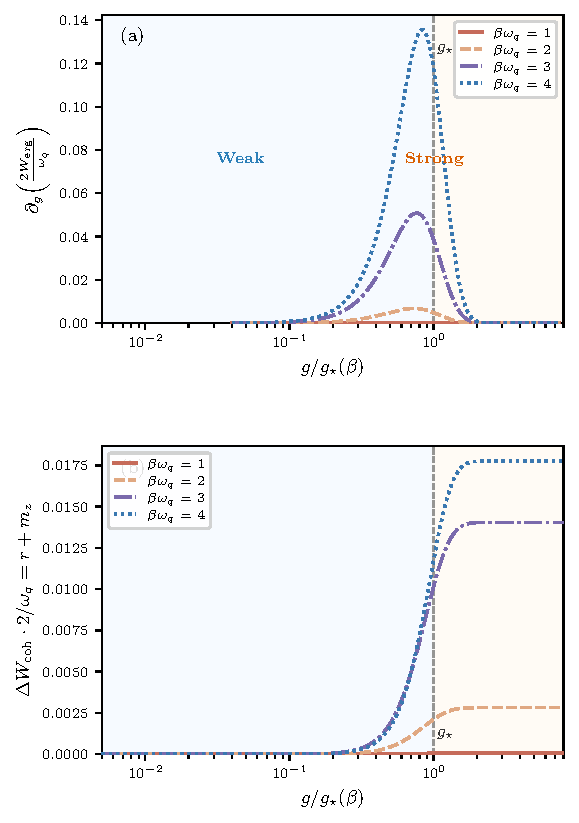
\includegraphics[width=\columnwidth]{../figures/hmf_ergotropy.pdf}
  \caption{Coherence-enabled ergotropy of the qubit mean-force state.
    \textbf{(a)} Ergotropy susceptibility
    $\partial_g \delta W_{\rm coh}$ versus $g/g_\star(\beta)$.
    The peak position locks near the crossover $g\approx g_\star$
    independent of temperature, while the peak height increases
    monotonically with $\beta$: low temperatures activate the
    transverse bath channel and make coherence-enabled work extraction
    increasingly efficient.
    \textbf{(b)} Coherence-enabled ergotropy
    $\delta W_{\rm coh}$ versus $g/g_\star(\beta)$ (calculated for $\omega_q=1$). Since $m_z<0$ throughout,
    $W_{\rm erg}(\delta[\rho])=0$ and $\delta W_{\rm coh}=W_{\rm erg}$
    in this regime. The onset occurs at the
    crossover and the saturation value grows with $\beta$,
    reflecting the increasing importance of the transverse bath
    channel $\Sigma_\perp$ at lower temperatures.}
  \label{fig:ergotropy}
\end{figure}

There is a final irony to this result.  While being most expolitable, this regime is simultaneously the most demanding for
numerical simulation.  Exact Diagonalisation (ED) of the truncated spin-boson
model faces two convergence requirements that become simultaneously binding
near $\chi\sim 1$.  On the spectral side, a faithful discretisation of $J(\omega)$
requires a mode count $N_\omega$ large enough to accurately quadrature the bath
kernel at $\omega\in\{0,\pm\omega_q\}$: at the crossover these integrals receive
comparable contributions from the full spectral window, so neither the infrared
nor the ultraviolet modes can be coarsened without systematic bias.  On the
state-space side, representing the polaron-like mean-force ground state demands
a per-mode Fock cutoff $n_{\max}\gtrsim\alpha_k^2$, where the mode displacement
$\alpha_k = g\,c_k/\omega_k$ is already appreciable at $g\sim g_\star(\beta)$
yet the state has not saturated to the simple displaced-vacuum structure it
acquires only at $\chi\gg 1$.  Neither the weak-coupling approximation nor the
ultrastrong polaron limit simplifies the representation, so both hierarchies
must be converged together.  The $\chi=1$ crossover partitions parameter
space into an ED-reliable sector ($\chi\lesssim 1$) and a
polaron-representability-limited sector ($\chi\gtrsim 1$), with the
susceptibility peaks sitting squarely on this boundary. 

 
\subsection{Ultrastrong duality and the Cresser--Anders limit}
\label{subsec:limits}

The ultrastrong regime $g\to\infty$ admits a strikingly clean interpretation
through the dual representation. In the direct chart, increasing the coupling
means the interaction Hamiltonian $H_{\rm int}=g\,f\otimes B$ overwhelms the
bare system Hamiltonian $H_Q$; the system's own energy levels become a
vanishing perturbation to the interacting system. But in the dual chart, the
roles are exchanged: the dual representation re-expresses the state as if
$H_Q$ were the dressing and the coupling basis the natural frame. Taking
$g\to\infty$ in the direct chart is therefore equivalent to taking $g\to 0$ in
the dual chart - the free-particle limit of the dual frame.

This inversion is visible directly in the symmetrised influence state.
At fixed $(\beta,\theta)$, the coupling-driven flow is
\begin{equation}
\begin{aligned}
\rho_S(g,\beta)
&=\frac{1}{2}\!\left(\mathbb I+r_S(g,\beta)\,
\hat{\mathbf m}_S(\beta,\theta)\!\cdot\!\boldsymbol{\sigma}\right),\\
r_S
&=\tanh\!\big(g^2\chi_0(\beta,\theta)\big).
\end{aligned}
\label{eq:rhoS_flow_v3}
\end{equation}
Because $\hat{\mathbf m}_S$ is $g$-independent, increasing $g$ traces a purely
radial flow: from the maximally mixed origin ($g=0$) to the boundary of the
Bloch disk ($g\to\infty$). In the direct chart,
Fig.~\ref{fig:ultrastrong_dual}(a), the different temperatures fan out toward
different attractors on the boundary, each set by the bath-dressed direction
$\hat{\mathbf m}_S(\beta)$. Crucially, these attractors are
\emph{temperature-dependent}: even at arbitrarily strong coupling the state
retains a memory of its temperature.

Applying the involutive duality map collapses this structure. The dual
influence state
\begin{equation}
\mathbf r_S^\vee
\,=\,\mathcal D_\beta[\mathbf r_S]
\label{eq:ca_dual_map}
\end{equation}
reorients each trajectory onto the coupling axis and rescales the radius by
the Cresser--Anders factor
$t_{\rm CA}(\beta)=\tanh(\beta\omega_q|\!\cos\theta|/2)$.
Figure~\ref{fig:ultrastrong_dual}(b) shows the result: the dual flows all
collapse onto a single ray along $\hat{\mathbf f}$, and the
$g\to\infty$ endpoints (squares) converge to the diamonds marking the
Cresser--Anders ultrastrong thermal
state~\cite{cresserWeakUltrastrongCoupling2021a},
\begin{equation}
\lim_{\lambda\to\infty}\rho_S
=\frac{1}{2}\left[\mathbb I-\sigma_{\hat{\mathbf f}}
\tanh\!\left(\frac{\beta\omega_q\cos\theta}{2}\right)\right].
\label{eq:ca_limit_qubit}
\end{equation}

The physical content of this convergence is immediate. In the ultrastrong
limit the bare system Hamiltonian is negligible; the equilibrium state is
diagonal in the coupling eigenbasis with an effective splitting
$\omega_q\cos\theta$ - the projection of the bare splitting onto the
coupling direction. The dual frame \emph{is} the coupling frame, and the
$g\to\infty$ limit in the direct representation maps to the uncoupled
($g\to 0$) limit of the dual, where the influence state is trivially thermal.
The Cresser--Anders result is thus not a separate calculation; it is the
zero-coupling asymptotic of the dual flow. Geometrically, the bath anisotropy
- the distinction between the resonant and non-resonant channels that
separately dress the Bloch vector - disappears in this limit, and the tilt
angle of the reduced state saturates at $\pi-\theta$: the Bloch vector aligns
with the coupling axis.

\begin{figure}[t]
    \centering
    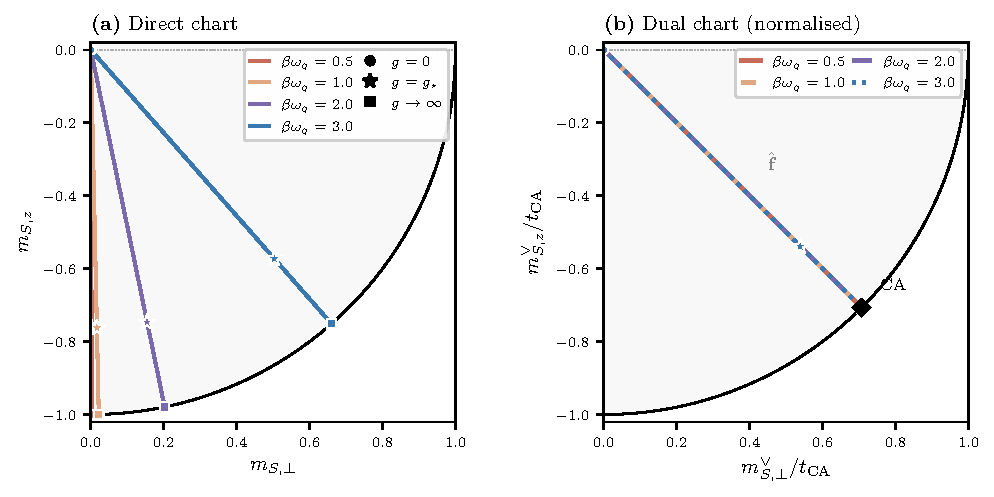
\includegraphics[width=\columnwidth]{../figures/hmf_ultrastrong_dual.pdf}
    \caption{Ultrastrong duality.
    \textbf{(a)}~Direct influence-state flows
    $\mathbf{r}_S(g)$ at fixed temperatures
    $\beta\omega_q\in\{0.5,1,2,3\}$ ($\theta=\pi/4$, Ohmic bath).
    Circles: $g=0$; stars: $g=g_\star$ (crossover); squares:
    $g\to\infty$. The flows fan toward temperature-dependent attractors.
    \textbf{(b)}~The same flows after the involutive dual map, normalised
    by $t_{\rm CA}(\beta)$. All trajectories collapse onto a single
    universal ray along $\hat{\mathbf f}$, with the $g\to\infty$ endpoints
    (squares) converging to the Cresser--Anders coupling-basis thermal
    state (diamond, $r=1$). The data collapse demonstrates that
    $g\to\infty$ in the direct chart is equivalent to $g\to 0$ in the
    dual: the free-particle limit of the dual frame.}
    \label{fig:ultrastrong_dual}
\end{figure}

